\section{PHÂN LỚP}

\subsection{Khái niệm}
Là bài toán phân loại trong đó cho sẵn bộ dữ liệu huấn luyện được cấu thành từ 1 cặp (x,y), trong đó x là các thuộc tính và y là nhãn lớp từ đó xây dựng mô hình . Nhiệm vụ là dùng mô hình đó để phân loại nhãn lớp cho mẫu dữ liệu.

\subsection{Các thuật ngữ chuyên ngành}
\begin{table}[H]
    \centering
    \renewcommand{\arraystretch}{1.3}
    \begin{tabularx}{\textwidth}{|p{4.5cm}|X|}
        \hline
        \textbf{Thuật ngữ (Tiếng Anh)} & \textbf{Diễn giải (Tiếng Việt)} \\
        \hline
        Instance / Sample & Mẫu dữ liệu: Một đối tượng cụ thể hoặc một dòng trong bảng dữ liệu. \\
        \hline
        Label & Nhãn mục tiêu: Kết quả phân loại hoặc danh mục mẫu thuộc về. \\
        \hline
        Training dataset & Tập huấn luyện: Phần dữ liệu có nhãn dùng để ``dạy'' mô hình học. \\
        \hline
        Testing dataset & Tập kiểm thử: Phần dữ liệu đánh giá độ chính xác của mô hình sau khi học. \\
        \hline
        Feature extraction & Trích xuất đặc trưng: Kỹ thuật tạo đặc điểm mới từ dữ liệu thô. \\
        \hline
        Feature selection & Lựa chọn đặc trưng: Chọn lọc thuộc tính quan trọng nhất. \\
        \hline
        Feature reduction & Giảm chiều dữ liệu: Giảm bớt số lượng biến số đầu vào. \\
        \hline
        Ground truth & Giá trị thực tế: Đáp án đúng tuyệt đối để đối chiếu kết quả. \\
        \hline
    \end{tabularx}
\end{table}

\subsection{Quy trình phân lớp}
\begin{figure}[H]
    \centering
    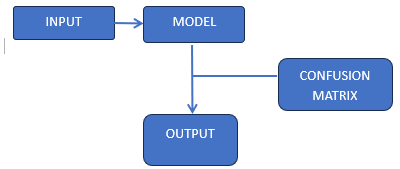
\includegraphics[width=1\textwidth]{figures/Classification/Classification_Process.png}
    \caption{Quy trình phân lớp}
    \label{fig:classification-process}
\end{figure}

Quy trình trong hình gồm hai giai đoạn. Ở giai đoạn huấn luyện, dữ liệu đã gán nhãn được tiền xử lý và dùng để xây dựng mô hình. Ở giai đoạn phân lớp, mô hình đã học nhận dữ liệu mới và dự đoán nhãn; nếu có nhãn thực tế, kết quả dự đoán được đối chiếu để đánh giá mô hình.

\subsection{Ví dụ và mô hình tổng quan}
\subsubsection*{5.1. Mô tả bài toán}
Xét bài toán dự đoán một học sinh có \textbf{đạt} bài kiểm tra hay không dựa trên hai thông tin: có đi học đầy đủ hay không và đã ôn bài hay chưa. Đây là bài toán phân lớp nhị phân với hai lớp \texttt{Yes} (đạt) và \texttt{No} (không đạt).

\subsubsection*{5.2. Mô tả dữ liệu}
Mỗi dòng là một mẫu học sinh. Hai cột ``Đi học đầy đủ'' và ``Ôn bài'' là các đặc trưng (features); cột ``Đạt bài kiểm tra'' là nhãn lớp (label). Bộ dữ liệu huấn luyện minh họa gồm ba mẫu:

\begin{table}[H]
    \centering
    \renewcommand{\arraystretch}{1.2}
    \begin{tabular}{|c|c|c|c|}
        \hline
        \textbf{Mẫu} & \textbf{Đi học đầy đủ} & \textbf{Ôn bài} & \textbf{Đạt bài kiểm tra (nhãn)} \\
        \hline
        1 & Yes & Yes & Yes \\
        \hline
        2 & Yes & No  & Yes \\
        \hline
        3 & No  & No  & No \\
        \hline
    \end{tabular}
    \caption{Ba mẫu dữ liệu huấn luyện cho ví dụ phân lớp}
    \label{tab:classification-simple-example}
\end{table}

\begin{figure}[H]
    \centering
    \begin{tikzpicture}[
        node distance=0.75cm and 0.8cm,
        box/.style={draw, rounded corners, align=center, minimum width=3.1cm, minimum height=1.05cm},
        arrow/.style={->, thick}
    ]
        \node[box] (data) {Dữ liệu huấn luyện\\3 mẫu, 2 đặc trưng, nhãn Yes/No};
        \node[box, right=of data] (train) {Huấn luyện\\mô hình phân lớp};
        \node[box, right=of train] (model) {Mô hình\\phân lớp};
        \node[box, below=of model] (predict) {Dự đoán nhãn\\Yes hoặc No};
        \node[box, left=of predict] (new) {Mẫu mới\\Đi học: Yes; Ôn bài: Yes};
        \draw[arrow] (data) -- node[above, align=center] {Học từ mẫu\\đã có nhãn} (train);
        \draw[arrow] (train) -- (model);
        \draw[arrow] (predict) -- (new);
        \draw[arrow] (model.south) -- ++(0,-0.35) -| node[pos=0, below] {áp dụng mô hình} (predict.north);
    \end{tikzpicture}
    \caption{Mô hình tổng quan của ví dụ phân lớp học sinh đạt hay không đạt}
    \label{fig:classification-simple-example}
\end{figure}
\subsubsection*{5.3. Nhiệm vụ phân lớp}
Từ ba mẫu đã biết nhãn, xây dựng mô hình học mối liên hệ giữa hai đặc trưng và kết quả kiểm tra. Sau đó, đưa đặc trưng của một học sinh mới vào mô hình để dự đoán nhãn \texttt{Yes} (đạt) hoặc \texttt{No} (không đạt). Với bảng minh họa trên, mẫu mới có ``Đi học đầy đủ = Yes'' và ``Ôn bài = Yes''; mô hình có thể dự đoán \texttt{Yes}.